\chapter{联合分布}

\section{随机向量}

\begin{definition}{联合CDF}{}
	$(X_1,\ldots,X_n):\Omega\to\RR^n$是($n$维)随机向量,$X_i$为随机变量。
	可定义联合CDF:
	\[
		\CDF(x_1,\ldots,x_n):=\P(X_1\leqslant x_1,\ldots,X_n\leqslant x_n),\quad(x_1,\ldots,x_n)\in\RR^n
	\]
	特别地,当$n=2$时,联合分布称为二元分布。
\end{definition}

\begin{definition}
	{离散分布}{}	
	若$X_i$均为离散型,则称$(X_1,\ldots,X_n)$为离散型随机向量。
\end{definition}

\begin{example}{多项分布}{multinomial distribution}
	给定$\Omega$的一个分割$\{B_1,\ldots,B_n\}$,$\P(B_i)=:p_i$,则 
	\[
		p_1+\cdots+p_n=1,
	\]
	独立试验$n$次,记$X_i=B_i$发生的次数,则$(X_1,\ldots,X_n)$服从多项分布(multinomial distribution),记作$(X_1,\ldots,X_n)\sim\Bino(n,p_1,\ldots,p_n)$,其联合PDF
	\begin{equation}
		\P(X_1=k_1,\ldots,X_n=k_n)=\binom{n}{k_1,\ldots,k_n}p_1^{k_1}\cdots p_n^{k_n}.
	\end{equation}
	其中多项式系数
	\begin{equation}
		\label{eq:multinomial coefficient}
		\binom{n}{k_1,\ldots,k_n}=\frac{n!}{k_1!\cdots k_n!},\quad k_1+\cdots+k_n=n,\quad k_i\geqslant 0.
	\end{equation}
	\begin{center}
		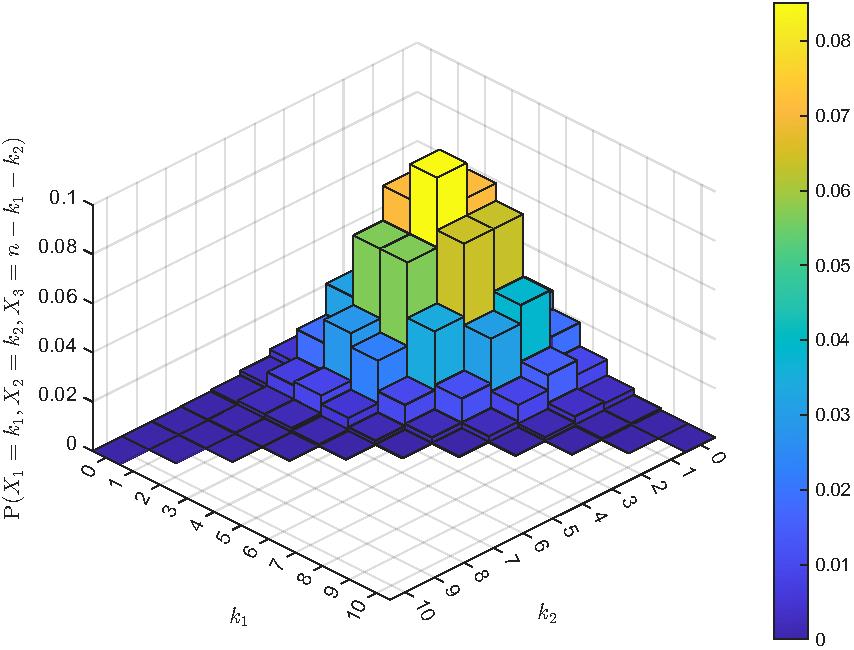
\includegraphics[width=.9\textwidth]{figures/pdf_bin3.pdf}
		\captionof{figure}{多项分布的例子:$(X_1,X_2,X_3)\sim\Bino(10,0.2,0.3,0.5)$}
		\label{fig:pdf_bin3}
	\end{center}
\end{example} 

\begin{definition}
	{连续分布}{}
	若存在$f\geqslant 0$且$\forall Q\subset\RR^n$可测,都有
	\[
		\P\bigkh{(X_1,\ldots,X_n)\in Q}=\int_Qf(x_1,\ldots,x_n)\d x_1\cdots\d x_n
	\]
	则称$(X_1,\ldots,X_n)$为连续型,且$f$为其PDF。
\end{definition}

\begin{corollary}
	连续分布相关性质:
	\begin{itemize}
		\item 归一性:
		\begin{equation}
			\int_{\RR^n}f(x_1,\ldots,x_n)\d x_1\cdots\d x_n\equiv 1;
		\end{equation}
		\item 以$n=2$为例,其CDF为
		\begin{subequations}
			\begin{align}
				\CDF(x,y)&=\int_{-\infty}^x\int_{-\infty}^yf(\xi,\eta)\d\xi\nd\eta,\\
				f(x,y)&=\pw{\CDF}xy(x,y).
			\end{align}
		\end{subequations}
	\end{itemize}
\end{corollary}

\begin{example}{二元矩形均匀分布}{2-D rectangle uniform distribution}
	矩形区域
	\[
		f(x,y)=\begin{cases}
			\frac1{(b-a)(c-d)},&(x,y)\in(a,b)\times(c,d)\\
			0,&\text{elsewhere}
		\end{cases}
	\]
\end{example}
\begin{example}{二元正态分布}{2-D normal distribution}
	$(X,Y)\sim\Norm(\mu_1,\mu_2,\sigma_1^2,\sigma_2^2,\rho)$,要求$\abs\rho<1$,其联合PDF为
	\begin{align}
		\begin{aligned}
			f(x,y)={}&\frac1{2\pi\sigma_1\sigma_2}\frac1{\sqrt{1-\rho^2}}\cdot\\
			&\exp\hkh{-\frac1{2(1-\rho^2)}\biggfkh{\biggkh{\frac{x-\mu_1}{\sigma_1}}^2+\biggkh{\frac{y-\mu_2}{\sigma_2}}^2-2\rho\frac{x-\mu_1}{\sigma_1}\frac{y-\mu_2}{\sigma_2}}}.
		\end{aligned}
	\end{align}
	特别地,标准二元正态分布为$(X,Y)\sim\Norm(1,1,0,0,0)$。
	\begin{center}
		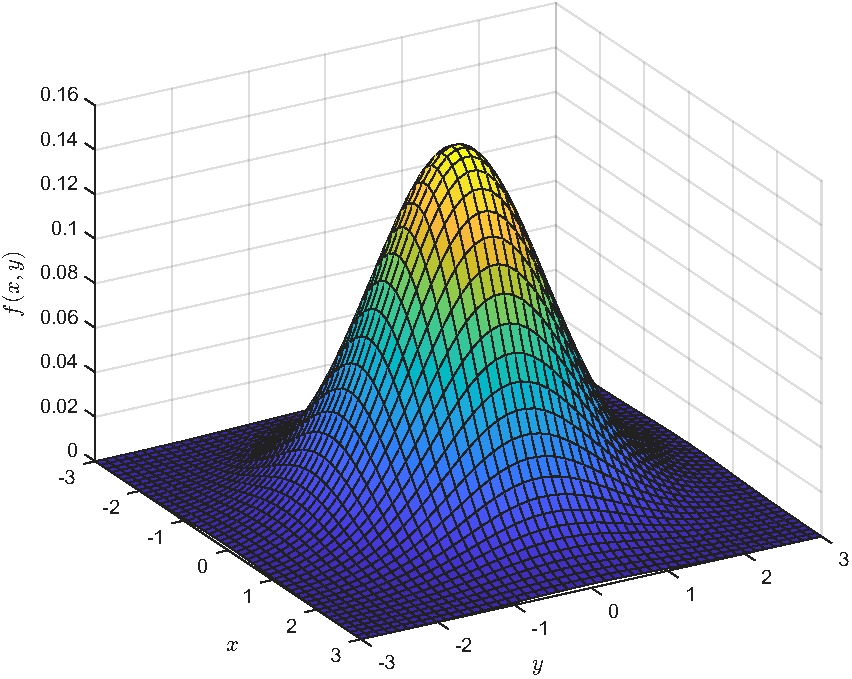
\includegraphics[width=.9\textwidth]{figures/pdf_norm2.pdf}
		\captionof{figure}{标准二元正态分布的PDF}
		\label{fig:pdf_norm2}
	\end{center}
	\tcblower
	指数项部分构成了一个二次型:$-X\tp WX/2$,其中
	\[
		X=\fkh{\frac{x-\mu_1}{\sigma_1},\frac{y-\mu_2}{\sigma_2}}\tp,\quad W=\frac1{1-\rho^2}\begin{bmatrix}
			1&-\rho\\-\rho&1
		\end{bmatrix}.
	\]
	对正定的$W$进行Cholesky分解$W=A\tp A$,可取
	\[
		A=\frac1{\sqrt{1-\rho^2}}\begin{bmatrix}
			1&-\rho\\0&\pm\sqrt{1-\rho^2}
		\end{bmatrix}
	\]
	进而就可将二次型转化为$\e{-(x^2+y^2)/2}$的标准形式。
\end{example}

\section{边际分布}

\begin{definition}{边际分布}{}
	$(X_1,\ldots,X_n)$中$X_i$的边际CDF
	\begin{equation}
		\CDF_{X_i}(x):=\P(X_i\leqslant x,\enspace X_{\neq i}\in\RR)
	\end{equation}
	以$n=2$为例,$(X,Y)$中$X$的边际CDF
	\[
		\CDF_X(x)=\lim_{y\to+\infty}\CDF(x,y)
	\]
	离散型边际概率
	\[
		\P(X=x)=\sum_y\P(X=x,Y=y);
	\]
	连续型边际PDF
	\[
		f_X(x)=\int\iti f(x,y)\d y.
	\]
\end{definition}

\begin{corollary}
	有 
	\[
		\P(X>a,Y>b)=1-\CDF_X(a)-\CDF_Y(b)+\CDF(a,b)
	\]
\end{corollary}

\begin{example}{二元正态的边际}{marginal PDF of 2-D normal distribution}
	边际密度
	\[
		f_X(x)=\int\iti f(x,y)\d y=\frac1{\sqrt{2\pi}\sigma_1}\exp\biggfkh{-\frac{(x-\mu_1)^2}{2\sigma_1^2}}.
	\]
	即$X\sim\Norm(\mu_1,\sigma_1^2)$,同理$Y\sim\Norm(\mu_2,\sigma_2^2)$。
\end{example}
\begin{remark}
	联合分布可确定边际分布,反之不行。
\end{remark}
\begin{example}{Farlie-Gumbel-Morgenstern族}{Farlie-Gumbel-Morgenstern family}
	随机变量$X,Y$的CDF分别为$\CDF(x),\mathrm G(y)$,则$\forall\alpha\in[-1,1],$
	\begin{equation}
		\mathrm H(x,y)=\CDF(x)\mathrm G(y)\bigfkh{1+\alpha\bigkh{1-\CDF(x)}\bigkh{1-\mathrm G(y)}}
	\end{equation}
	是$(X,Y)$的二元CDF。且$X,Y$的边际分布分别为$\CDF(x),\mathrm G(y)$。
\end{example}
\begin{example}{连接函数}{Copula function}
	我们称边际分布为$\Unif(0,1)$的联合CDF $\mathrm C(u,v)$为连接(Copula)函数,则对于随机变量$X,Y$,可用连接函数构造二元分布
	\begin{equation}
		\mathrm H(x,y)=\mathrm C\bigkh{\CDF(x),\mathrm G(y)}
	\end{equation}
	使其边际CDF为$\CDF(x),\mathrm G(y)$。
\end{example}

\section{条件分布}

\begin{definition}
	{条件分布}{}
	以$n=2$为例,离散型
	\[
		\P(X=x_i,Y=y_j)=:p_{ij}\geqslant 0,\quad\sum_{i,j}p_{ij}=1,
	\]
	有条件概率
	\begin{equation}
		\P(X=x_i|Y=y_i)=\frac{\P(X=x_i,Y=y_i)}{\P(Y=y_i)}=\frac{p_{ij}}{\sum_kp_{kj}}=:\frac{p_{ij}}{p_{\cdot j}}.
	\end{equation}
	
	连续型PDF为$f(x,y)$,
	%\P(X\leqslant x|y<Y\leqslant y+\d y)=\dvd{\int_{-\infty}^x\int_y^{y+\d y}f(\xi,\eta)\d\eta\nd\xi}{\int_y^{y+\d y}f(\xi,\eta)\d\eta}
	可定义条件PDF\footnote{唐宏岩老师记作$f_X(x|y)$}
	\begin{equation}
		f_{X|Y}(x|y)=\frac{f(x,y)}{f_Y(y)}.
	\end{equation}
	条件CDF
	\[
		\CDF(a|y)=\P(X\leqslant a|Y=y)=\int_{-\infty}^af_{X|Y}(x|y)\d x.
	\]%不能用条件PDF计算,因为$Y=y$概率为0,应当直接积分
\end{definition}

\begin{corollary}
	乘法法则
	\begin{equation}
		f(x,y)=f_Y(y)f_{X|Y}(x|y)=f_X(x)f_{Y|X}(y|x);
	\end{equation}
	全概率公式 
	\begin{equation}
		f_X(x)=\int\iti f_{X|Y}(x|y)f_Y(y)\d y;
	\end{equation}
	Bayes公式 
	\begin{equation}
		f_{Y|X}(y|x)=\frac{f_{X|Y}(x|y)f_Y(y)}{f_X(x)}.
	\end{equation}
\end{corollary}

\begin{example}{二元正态的条件密度}{conditional PDF of 2-D normal distribution}
	$X,Y\sim\Norm(\mu_1,\mu_2,\sigma_1^2,\sigma_2^2,\rho)$
	\begin{equation}
		f_{Y|X}(y|x)=\frac1{\sqrt{2\pi}\sigma_2}\frac1{\sqrt{1-\rho^2}}\exp\biggfkh{-\frac1{2(1-\rho^2)}\Bigkh{\frac{y-\mu_2}{\sigma_2}-\rho\frac{x-\mu_1}{\sigma_1}}^2},
	\end{equation}
	当$X=x$时,$Y\sim\Norm\Bigkh{\mu_2+\rho\frac{\sigma_2}{\sigma_1}(x-\mu_1),(1-\rho^2)\sigma_2^2}$
\end{example}

\section{独立性}

\begin{definition}{联合分布的独立性}{}
	定义$(X,Y)$的CDF为$\CDF(x,y)$,定义$X,Y$独立满足
	\begin{equation}
		\CDF(x,y)=\CDF_X(x)\CDF_X(y),\quad\forall x,y\in\RR
	\end{equation}
	进而定义$X_1,\ldots,X_n$独立: 
	\[
		\CDF(x_1,\ldots,x_n)=\CDF_1(x_1)\cdots\CDF(x_n),\quad\forall x_1,\ldots,x_n\in\RR
	\]
\end{definition}
\begin{corollary}
	离散型中,即
	\[
		p_{ij}=p_{i\cdot}p_{\cdot j},\quad \forall i,j
	\]
	连续型中,即
	\[
		f(x,y)=f_X(x)f_Y(y),\quad \forall x,y\in\RR
	\]
\end{corollary}
\begin{example}{二元正态分布的独立性}{}
	若$(X,Y)\sim\Norm(\mu_1,\mu_2,\sigma_1^2,\sigma_2^2,\rho)$,则$X,Y$独立$\iff\rho=0.$
\end{example}


\begin{theorem}{独立性相关定理}{independent}
	\begin{compactenum}
		\item 若$X_1,\ldots,X_n$独立,则
		\[
			Y_1=g_1(X_1,\ldots,X_m),\quad Y_2=g_2(X_{m+1},\ldots,X_n)
		\]
		独立;
		\item 若联合PDF可以分离变量
		\[
			f(x_1,\ldots,x_n)=g_1(x_1)\cdots g_n(x_n),\quad x_1,\ldots,x_n\in\RR
		\]
		则$X_1,\ldots,X_n$相互独立,且$g_i(x_i)\propto f_i(x_i)$相差常数因子。
	\end{compactenum}
\end{theorem}

\section{随机向量的函数}

\begin{theorem}
	{密度函数变换}{}
	$(X,Y)$为二维连续型随机变量,其PDF为$f_{X,Y}(x,y)$。由此可导出随机变量$(U,V)=\bigkh{u(X,Y),v(X,Y)}$,求其PDF $f_{U,V}(u,v)$。
	
	仅考虑$u,v$可微可逆:
	\[
		\begin{cases}
			u=u(x,y)\\
			v=v(x,y)
		\end{cases}\iff
		\begin{cases}
			x=x(u,v)\\
			y=y(u,v)
		\end{cases}
	\]
	则该变换的Jacobi行列式
	\[
		\det J=\abs{\pv{(x,y)}{(u,v)}}=\begin{vmatrix}
			x_u&y_u\\x_v&y_v
		\end{vmatrix}\neq 0
	\]
	则$U,V$的联合分布PDF为
	\begin{equation}
		\label{UVXY}
		f_{U,V}(u,v)=f_{X,Y}\bigfkh{x(u,v),y(u,v)}\abs{\det J}.
	\end{equation}
\end{theorem}
\begin{remark}
	特别需要注意是否有“一对多”的情况,比如$(U,V)=(X^2+Y^2,X/Y)$。
\end{remark}
\begin{example}{$X+Y$}{X+Y}
	$(X,Y)$的和$Z=X+Y$的PDF为
	\begin{equation}
		f_{X+Y}(z)=\int\iti f(x,z-x)\d x\equiv\int\iti f(z-y,y)\d y
	\end{equation}
	特别地,当$X,Y$相互独立时,%若其边缘分布PDF分别为$f_X,f_Y$,则
	\[
		f_{X+Y}(z)=\int\iti f_X(x)f_Y(z-x)\d x\equiv\int\iti f_X(z-y)f_Y(y)\d y
	\]
	这是$f_X,f_Y$的Fourier卷积,记作$f_X\ast f_Y$。
\end{example}
\begin{remark}
	可构造辅助随机变量$(Z,W)=(X+Y,X)$,用式\eqref{UVXY}得出。
\end{remark}
\begin{example}{$Y/X,XY$}{Y/X,XY}
	$Z=Y/X,XY$的PDF为
	\begin{subequations}
		\begin{align}
			f_{Y/X}(z)&=\int\iti f_{X,Y}(x,xz)\abs x\d x\\
			f_{XY}(z)&=\int\iti f_{X,Y}\biggkh{x,\frac zx}\frac1{\abs{x}}\d x
		\end{align}
	\end{subequations}
	特别地,当$X,Y$相互独立时,
	\begin{subequations}
		\begin{align}
			f_{Y/X}(z)&=\int\iti f_X(x)f_Y(xz)\abs x\d x\\
			f_{XY}(z)&=\int\iti f_X(x)f_Y\kh{\frac zx}\frac1{\abs x}\d x
		\end{align}
	\end{subequations}
	第二个公式是$f_X,f_Y$的Mellin卷积。
\end{example}
\begin{example}{$\max(X,Y),\min(X,Y)$}{max,min}
	若$(X,Y)$独立,则$\max(X,Y),\min(X,Y)$的分布为
	\begin{subequations}
		\label{eq:min-max distribution}
		\begin{align}
			\CDF_{\max{}}(z)&=\CDF_X(x)\CDF_Y(y),\\
			\CDF_{\min{}}(z)&=1-[1-\CDF_X(x)][1-\CDF_Y(y)].
		\end{align}
	\end{subequations}
	上式很容易推导:
	\[
		\P(\max(X,Y)<z)=\P(X<z,Y<z)=\P(X<z)\P(Y<z),
	\]
\end{example}
\begin{example}{离散分布的和}{sum of discrete distribution}
	$X_i\sim\Bino(n_i,p)$独立,和$X_1+X_2$
	\begin{align*}
		\P(X_1+X_2=k)&=\sum_{k_1=0}^k\P(X_1=k_1,X_2=k-k_1)\\
		&=\sum_{k_1=0}^k\binom{n_1}{k_1}\binom{n_2}{k-k_1}p^k(1-p)^{n_1+n_2-k}\\
		&=\binom{n_1+n_2}{k}p^k(1-p)^{n_1+n_2-k}
	\end{align*}
	故$X_1+X_2\sim\Bino(n_1+n_2,p).$
	\tcblower
	$X_i\sim\Pois(\lambda_i)$独立,和$X_1+X_2$
	\begin{align*}
		\P(X_1+X_2=k)&=\sum_{k_1=0}^k\frac{\lambda_1^{k_1}}{k_1!}\e{-\lambda_1}\frac{\lambda_2^{k-k_1}}{(k-k_1)!}\e{-\lambda_2}\\
		&=\frac{\e{-(\lambda_1+\lambda_2)}}{k!}\sum_{k_1=0}^k\binom{k}{k_1}\lambda_i^{k_1}\lambda_2^{k-k_1}\\
		&=\frac{\e{-(\lambda_1+\lambda_2)}}{k!}(\lambda_1+\lambda_2)^k
	\end{align*}
	故$X_1+X_2\sim\Pois(\lambda_1+\lambda_2).$
\end{example}
\begin{remark}
	在学习到矩母函数和特征函数后,由\thmref{thm:the distribution of the sum of the independent random variable},这个结论就是显然的。
\end{remark}
\begin{example}{正态分布的和}{sum of continuous distribution}
	$(X_1,X_2)\sim\Norm(\mu_1,\mu_2,\sigma_1^2,\sigma_2^2,\rho),\enspace Y=X_1+X_2$,
	\[
		f(y)=\int\iti f(x, y-x)\d x=\cdots
	\]
	故$Y=X_1+X_2\sim\Norm(\mu_1+\mu_2,\sigma_1^2+\sigma_1^2+2\rho\sigma_1\sigma_2).$
\end{example}
\begin{example}{指数分布的最小值}{}
	若$X_1\sim\Expo(\lambda_1),X_2\sim\Expo(\lambda_2)$,则 
	\[
		\CDF_{\min{}}(x)=1-\bigfkh{1-\CDF_{X_1}(x)}\bigfkh{1-\CDF_{X_2}(x)}=1-\e{-(\lambda_1+\lambda_2)x}.
	\]
	$\min(X_1,X_2)\sim\Expo(\lambda_1+\lambda_2).$
\end{example}
\begin{example}{max, min的联合分布}{min-max joint distribution}
	$X_1,\ldots,X_n$独立同分布(independent identically distribution, iid\index{iid, 独立同分布}),其CDF为$\CDF(x)$。

	求$Y:=\min(X_1,\ldots,X_n)$和$Z:=\max(X_1,\ldots,X_n)$的联合分布。
	由
	\[
		\P(y<Y,Z\leqslant z)=\P(y<X_i\leqslant z)=\bigfkh{\CDF(z)-\CDF(y)}^n.
	\]
	另一方面$\P(y<Y,Z\leqslant z)=\CDF_Z(z)-\CDF_{Y,Z}(y,z)$,
	故
	\begin{equation}
		\label{eq:min-max joint distribution}
		f_{Y,Z}(y,z)=-\frac{\partial^2}{\partial y \partial z}\P(y<Y,Z\leqslant z)=n(n-1)f(y)f(z)\bigfkh{\CDF(z)-\CDF(y)}^{n-2}.
	\end{equation}
\end{example}

\section{三大分布}
\label{subsec:chi2, t, F}

\begin{definition}{卡方分布}{chi-square distribution}
	若$X_1,\ldots,X_n$ iid $\sim\Norm(0,1)$ ,则$X:=X_1^2+\cdots+X_n^2$服从自由度为$n$的卡方分布,记作$X\sim\chi^2(n)$,由数学归纳法可知
	\begin{equation}
		f(x)=\frac1{\Gamma(n/2)2^{n/2}}x^{n/2-1}\e{-x/2},\quad x>0.
	\end{equation}
	\begin{center}
		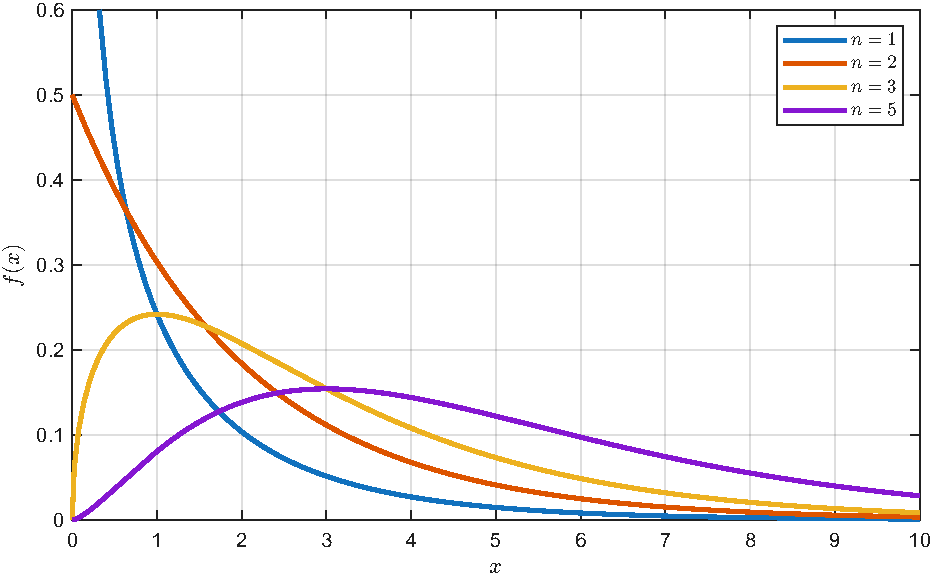
\includegraphics[width=0.8\linewidth]{figures/pdf_chi2.pdf}
		\captionof{figure}{卡方分布的PDF}
		\label{fig:pdf_chi2}
	\end{center}
\end{definition}

\begin{corollary}
	卡方分布的期望和方差
	\begin{subequations}
		\begin{align}
			\E(X) &= n,\\
			\Var(X) &= 2n.
		\end{align}
	\end{subequations}
\end{corollary}

\begin{corollary}
	若$X_1\sim\chi^2(n_1),X_2\sim\chi^2(n_2)$独立,则$X_1+X_2\sim\chi^2(n_1+n_2);$
\end{corollary}

\begin{corollary}
	若$X\sim\Expo(\lambda)$,则$2\lambda X\sim\chi^2(2).$
\end{corollary}

\begin{definition}{Student's t分布}{Student's t distribution}
	$X_1\sim\chi^2(n),X_2\sim\Norm(0,1)$独立,则可构造t分布:
	\[
		X:=\frac{X_2}{\sqrt{X_1/n}}\sim\mathrm t(n).
	\]
	其PDF为
	\begin{equation}
		f(x)=\frac1{\sqrt n\mathrm B(n/2,1/2)}\biggkh{1+\frac{x^2}n}^{-(n+1)/2},\quad x\in\RR.
	\end{equation}
	特别地,当$n=1$时,是Cauchy分布;$n\to\infty$时,趋于$\Norm(0,1)$。
	事实上,由\figref{fig:pdf_t} 可见,$n=30$时二者已经非常接近。
	\begin{center}
		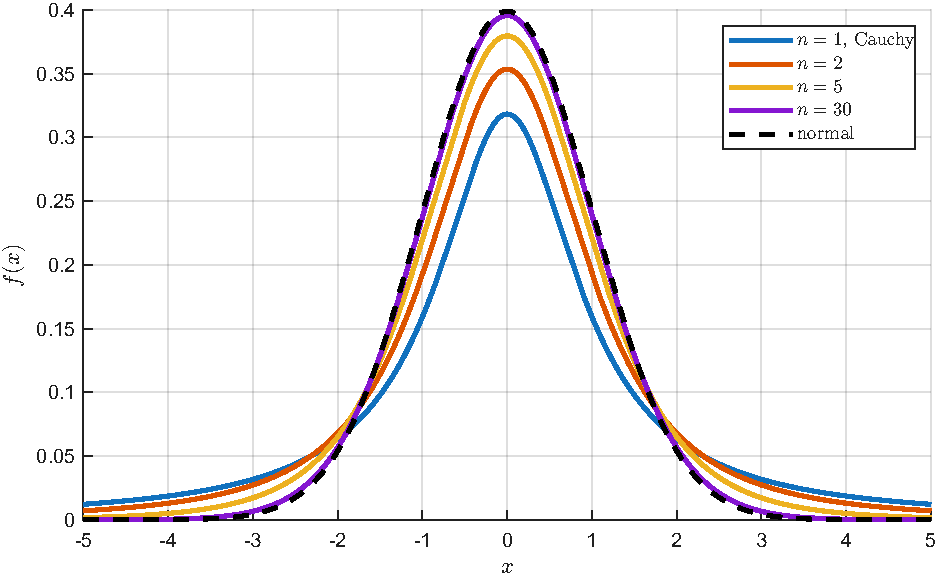
\includegraphics[width=0.8\linewidth]{figures/pdf_t.pdf}
		\captionof{figure}{t分布的PDF}
		\label{fig:pdf_t}
	\end{center}
\end{definition}

\begin{corollary}
	t分布的期望和方差
	\begin{subequations}
		\begin{align}
			E(X)&=0,\\
			\Var(X)&=\frac{n}{n-2}.
		\end{align}
	\end{subequations}
	当$n=1,2$时,方差不存在。
\end{corollary}

\begin{definition}{F分布}{F distribution}
	$X_1\sim\chi^2(n_1),X_2\sim\chi^2(n_2)$独立,则可构造F分布:
	\[
		X:=\frac{X_1/n_1}{X_2/n_2}\sim\mathrm F(n_1,n_2).
	\]
	其PDF为
	\begin{equation}
		f(x)=\frac1{\mathrm B(n_1/2,n_2/2)}\Bigkh{\frac{n_1}{n_2}}^{n_1/2}x^{n_1/2-1}\Bigkh{1+\frac{n_1}{n_2}x}^{-(n_1+n_2)/2},\quad x>0.
	\end{equation}
	\begin{center}
		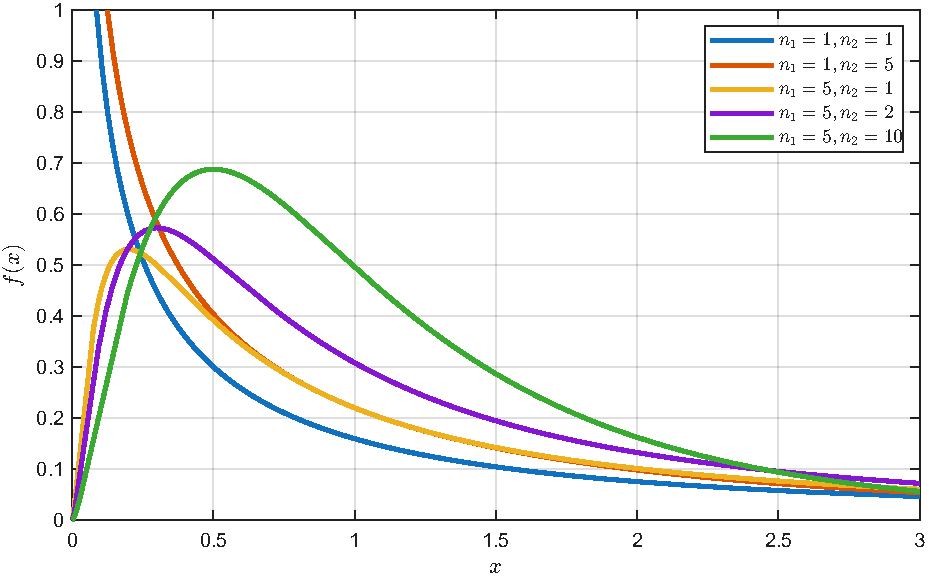
\includegraphics[width=0.8\linewidth]{figures/pdf_F.pdf}
		\captionof{figure}{F分布的PDF}
		\label{fig:pdf_F}
	\end{center}
\end{definition}

\begin{corollary}
	F分布的期望和方差
	\begin{subequations}
		\begin{align}
			E(X)&=\frac{n_2}{n_2-2},\quad n_2>2,\\
			\Var(X)&=\frac{2n_2^2(n_1+n_2-2)}{n_1(n_2-2)^2(n_2-4)},\quad n_2>4.
		\end{align}
	\end{subequations}
\end{corollary}

% \begin{corollary}
% 	若$X\sim\mathrm F(n_1,n_2)$,则$1/X\sim\mathrm F(n_2,n_1)$。
% \end{corollary}

% \begin{corollary}
% 	若$X\sim\mathrm t(n)$,则$X^2\sim\mathrm F(1,n)$。
% \end{corollary}

\begin{theorem}{正态总体统计量的分布}{the distribution of normal statistic}
	$X_1\ldots,X_n$ iid $\sim\Norm(\mu,\sigma^2)$,$X_1',\ldots,X_{n'}'$ iid $\sim\Norm(\mu',\sigma'^2)$,则
	\begin{subequations}
		\begin{align}
			\label{sample-N}
			\frac{\avg X-\mu}{\sigma/\sqrt n}&\sim\Norm(0,1);\\
			\label{sample-chi2}
			\frac{(n-1)S^2}{\sigma^2}&\sim\chi^2(n-1);\\
			\label{sample-t}
			\frac{\avg X-\mu}{S/\sqrt n}&\sim\mathrm t(n-1);\\
			\label{2sample-F}
			\frac{S^2/S'^2}{\sigma^2/\sigma'^2}&\sim\mathrm F(n-1,n'-1).
		\end{align}
	\end{subequations}
\end{theorem}
\begin{proof}
	式\eqref{sample-N}是trivial的,因为$\avg X\sim\Norm(\mu,\sigma^2/n).$
	
	式\eqref{sample-t}可由式\eqref{sample-chi2}, \eqref{sample-N}结合t分布的定义推导出来
	\[
		\frac{\avg X-\mu}{S/\sqrt n}=\division{\frac{\avg X-\mu}{\sigma/\sqrt n}}{\sqrt{\frac{(n-1)S^2/\sigma^2}{n-1}}}\sim\mathrm t(n-1),
	\]
	式\eqref{2sample-F}也可由式\eqref{sample-chi2}结合F分布的定义推导而来,因此只需证明式\eqref{sample-chi2}即可。

	$(X_1,\ldots,X_n)$的PDF为
	\[
		f(x_1,\ldots,x_n)=\frac1{(\sqrt{2\pi}\sigma)^n}\exp\biggfkh{-\frac1{2\sigma^2}\biggkh{\sum_{i=1}^nx_i^2-2\mu\sum_{i=1}^nx_i+n\mu^2}}.
	\]
	我们希望构造另一个独立随机向量$(Y_1,\ldots,Y_n)$,使$Y_1$与$Y_2^2+\cdots+Y_n^2$的关系类似$\avg X$与$S^2$。为满足独立性,可以要求变换
	\[
		\begin{bmatrix}
			Y_1\\\vdots\\Y_n
		\end{bmatrix}=A\begin{bmatrix}
			X_1\\\vdots\\X_n
		\end{bmatrix}.
	\]
	是正交的,我们还可以额外要求正交方阵$A$的第一行各元均为$1/\sqrt n$,由于$A$的各行相当于$\RR^n$中的一组正交归一基,因此这总可以通过Gram-Schmidt过程满足。
	由此
	\[
		\sum_{i=1}^nY_i^2=\sum_{i=1}^nX_i^2,\quad Y_1=\frac1{\sqrt n}\sum_{i=1}^nX_i\equiv\sqrt n\,\avg X.
	\]
	从而,$(Y_1,\ldots,Y_n)$的PDF
	\begin{align*}
		f(y_1,\ldots,y_n)&=\frac1{(\sqrt{2\pi}\sigma)^n}\exp\biggfkh{-\frac1{2\sigma^2}\biggkh{\sum_{i=1}^ny_i^2-2\mu\sqrt ny_1+n\mu^2}}\\
		&=\frac1{\sqrt{2\pi}\sigma}\e{-(y_1-\sqrt n\mu)^2/2\sigma^2}\cdot\frac1{\sqrt{2\pi}\sigma}\e{-y_2^2/2\sigma^2}\cdots\frac1{\sqrt{2\pi}\sigma}\e{-y_n^2/2\sigma^2}.
	\end{align*}
	故$Y_1,\ldots,Y_n$独立,且
	\[
		Y_1\sim\Norm(\sqrt n\mu,\sigma^2),\quad Y_i\sim\Norm(0,\sigma^2),\enspace i=2,\ldots,n.
	\]
	从而$Y_1$与$Y_2^2+\cdots+Y_n^2$独立,又
	\[
		\sum_{i=2}^nY_i^2=\sum_{i=1}^nY_i^2-Y_1^2=\sum_{i=1}^nX_i^2-n\avg X^2=\sum_{i=1}^n(X_i-\avg X)^2.
	\]
	故$\avg X$与$S^2$独立,且
	\[
		\frac{(n-1)S^2}{\sigma^2}=\frac1{\sigma^2}\sum_{i=1}^n(X_i-\avg X)^2=\frac1{\sigma^2}\sum_{i=2}^nY_i^2\sim\chi^2(n-1).
		\qedhere
	\]
\end{proof}